\documentclass[aspectratio=169]{beamer}

\mode<presentation>
{
  \usetheme{default}
  \usecolortheme{default}
  \usefonttheme{default}
  \setbeamertemplate{navigation symbols}{}
  \setbeamertemplate{caption}[numbered]
  \setbeamertemplate{footline}[frame number]  % or "page number"
  \setbeamercolor{frametitle}{fg=white}
  \setbeamercolor{footline}{fg=black}
} 

\usepackage[english]{babel}
\usepackage[utf8x]{inputenc}
\usepackage{tikz}
\usepackage{courier}
\usepackage{array}
\usepackage{bold-extra}
\usepackage{minted}
\usepackage[thicklines]{cancel}

\xdefinecolor{dianablue}{rgb}{0.18,0.24,0.31}
\xdefinecolor{darkblue}{rgb}{0.1,0.1,0.7}
\xdefinecolor{darkgreen}{rgb}{0,0.5,0}
\xdefinecolor{darkdarkgreen}{rgb}{0,0.4,0}
\xdefinecolor{darkgrey}{rgb}{0.35,0.35,0.35}
\xdefinecolor{darkorange}{rgb}{0.8,0.5,0}
\xdefinecolor{darkred}{rgb}{0.7,0,0}
\definecolor{darkgreen}{rgb}{0,0.6,0}
\definecolor{mauve}{rgb}{0.58,0,0.82}

\title[2017-12-13-ieee-bigdata]{Fast Access to Columnar, Hierarchical Data \\ via Code Transformation}
\author{Jim Pivarski$^1$, Peter Elmer$^1$, Brian Bockelman$^2$, and Zhe Zhang$^2$}
\institute{$^1$Princeton University, $^2$University of Nebraska at Lincoln -- DIANA-HEP}
\date{December 13, 2017}

\begin{document}

\logo{\pgfputat{\pgfxy(0.11, 7.4)}{\pgfbox[right,base]{\tikz{\filldraw[fill=dianablue, draw=none] (0 cm, 0 cm) rectangle (50 cm, 1 cm);}\mbox{\hspace{-9 cm}
\includegraphics[height=1 cm]{princeton-logo-long.png}
\includegraphics[height=1 cm]{nebraska-logo-long.png}
\includegraphics[height=1 cm]{diana-hep-logo-long.png}}}}}

\begin{frame}
  \titlepage
\end{frame}

\logo{\pgfputat{\pgfxy(0.11, 7.4)}{\pgfbox[right,base]{\tikz{\filldraw[fill=dianablue, draw=none] (0 cm, 0 cm) rectangle (50 cm, 1 cm);}\mbox{\hspace{-8 cm}
\includegraphics[height=1 cm]{princeton-logo.png}
\includegraphics[height=1 cm]{nebraska-logo.png}
\includegraphics[height=1 cm]{diana-hep-logo.png}}}}}

% Uncomment these lines for an automatically generated outline.
%\begin{frame}{Outline}
%  \tableofcontents
%\end{frame}

% START START START START START START START START START START START START START

%% \begin{frame}{My sliding definition of ``big data''}
%% \vspace{0.5 cm}
%% \begin{center}
%% \Large {\bf Big data (n.):} Techniques for handling datasets that are too big for a single computer.

%% \vspace{1 cm}
%% \uncover<2->{\textcolor{darkblue}{This is a moving target: different sizes in different decades.}}
%% \end{center}
%% \end{frame}

%% \begin{frame}{}

%% \begin{columns}
%% \column{1.15\linewidth}
%% 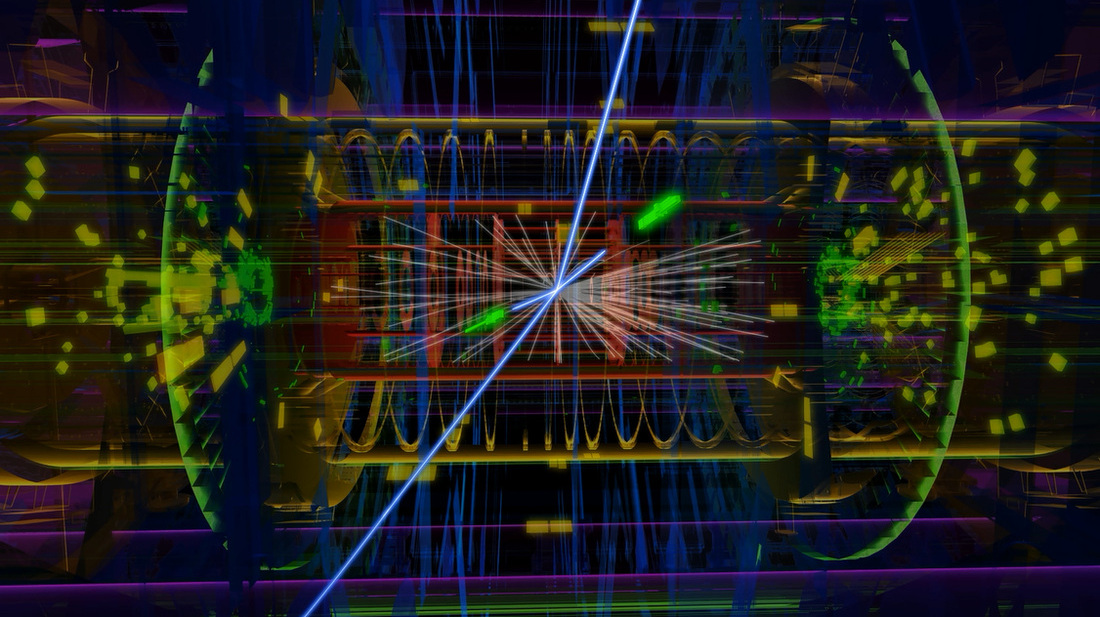
\includegraphics[width=\linewidth]{complex-atlas-collision-art.jpg}
%% \end{columns}

%% \vspace{-8.2 cm}
%% \uncover<1->{\textcolor{white}{\huge\bf In that sense, high-energy physicists have always dealt with big data.}}
%% \vspace{8.2 cm}
%% \end{frame}

%% \begin{frame}{High-energy physicists have always dealt with big data}
%% \vspace{0.5 cm}
%% \only<1>{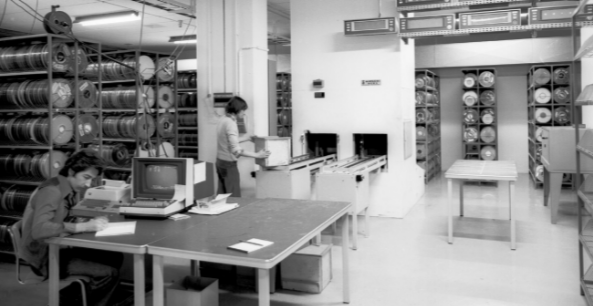
\includegraphics[width=\linewidth]{tapes1.png}}
%% \only<2>{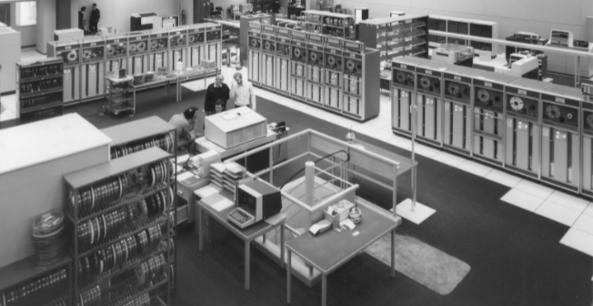
\includegraphics[width=\linewidth]{tapes2.png}}
%% \only<3>{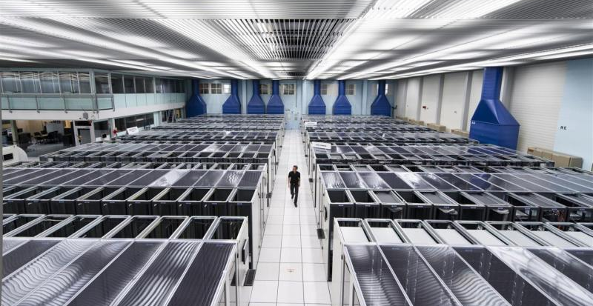
\includegraphics[width=\linewidth]{cerncomputing.png}}
%% \end{frame}

%% \begin{frame}{But we're certainly not the leaders in big data anymore}
%% \vspace{0.35 cm}
%% 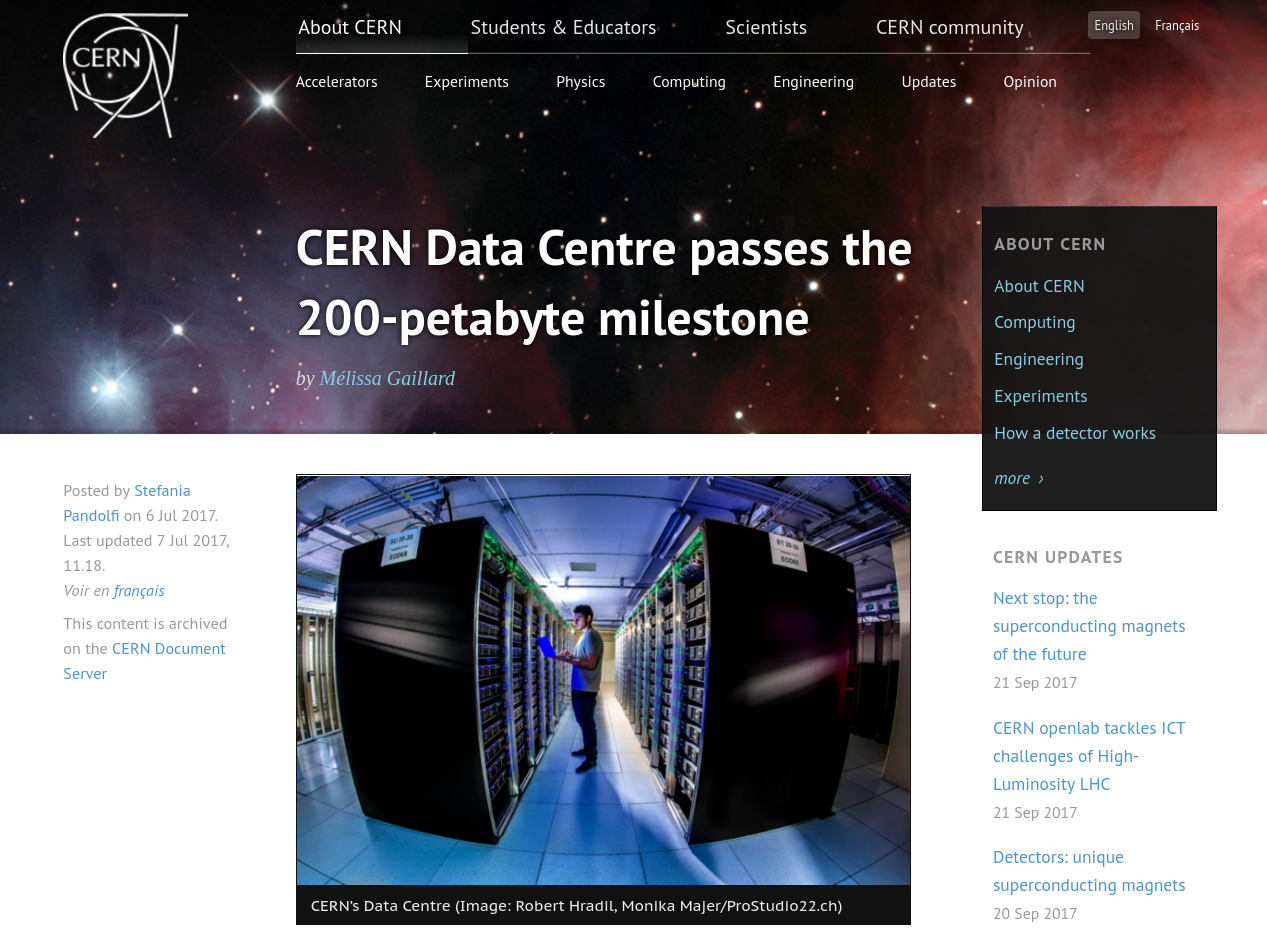
\includegraphics[width=0.73\linewidth]{cern-200pb.png}

%% \vspace{-4.8 cm}
%% \uncover<2->{\mbox{ } \hfill 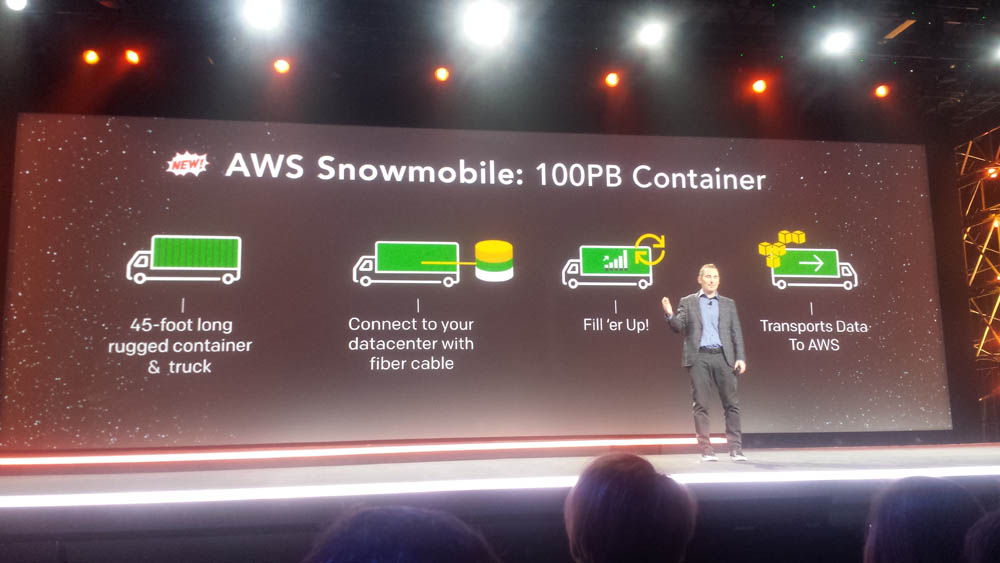
\includegraphics[width=0.7\linewidth]{aws-snowmobile.jpg}\hspace{-1 cm}}
%% \end{frame}

%% \begin{frame}{Data structure management in high-energy physics}
%% \vspace{0.25 cm}
%% 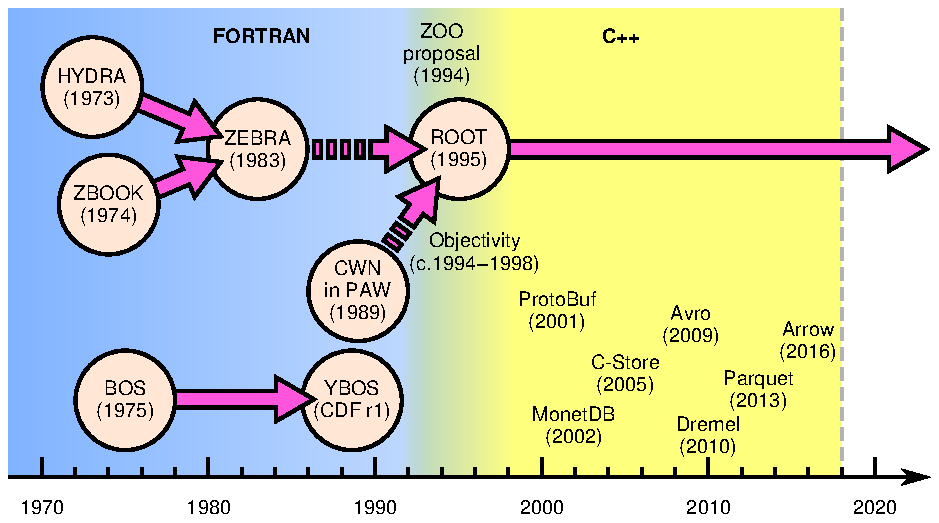
\includegraphics[width=\linewidth]{history.pdf}
%% \end{frame}

%% \begin{frame}[fragile]{High-energy physics data are arbitrary length lists}
%% \vspace{0.25 cm}
%% 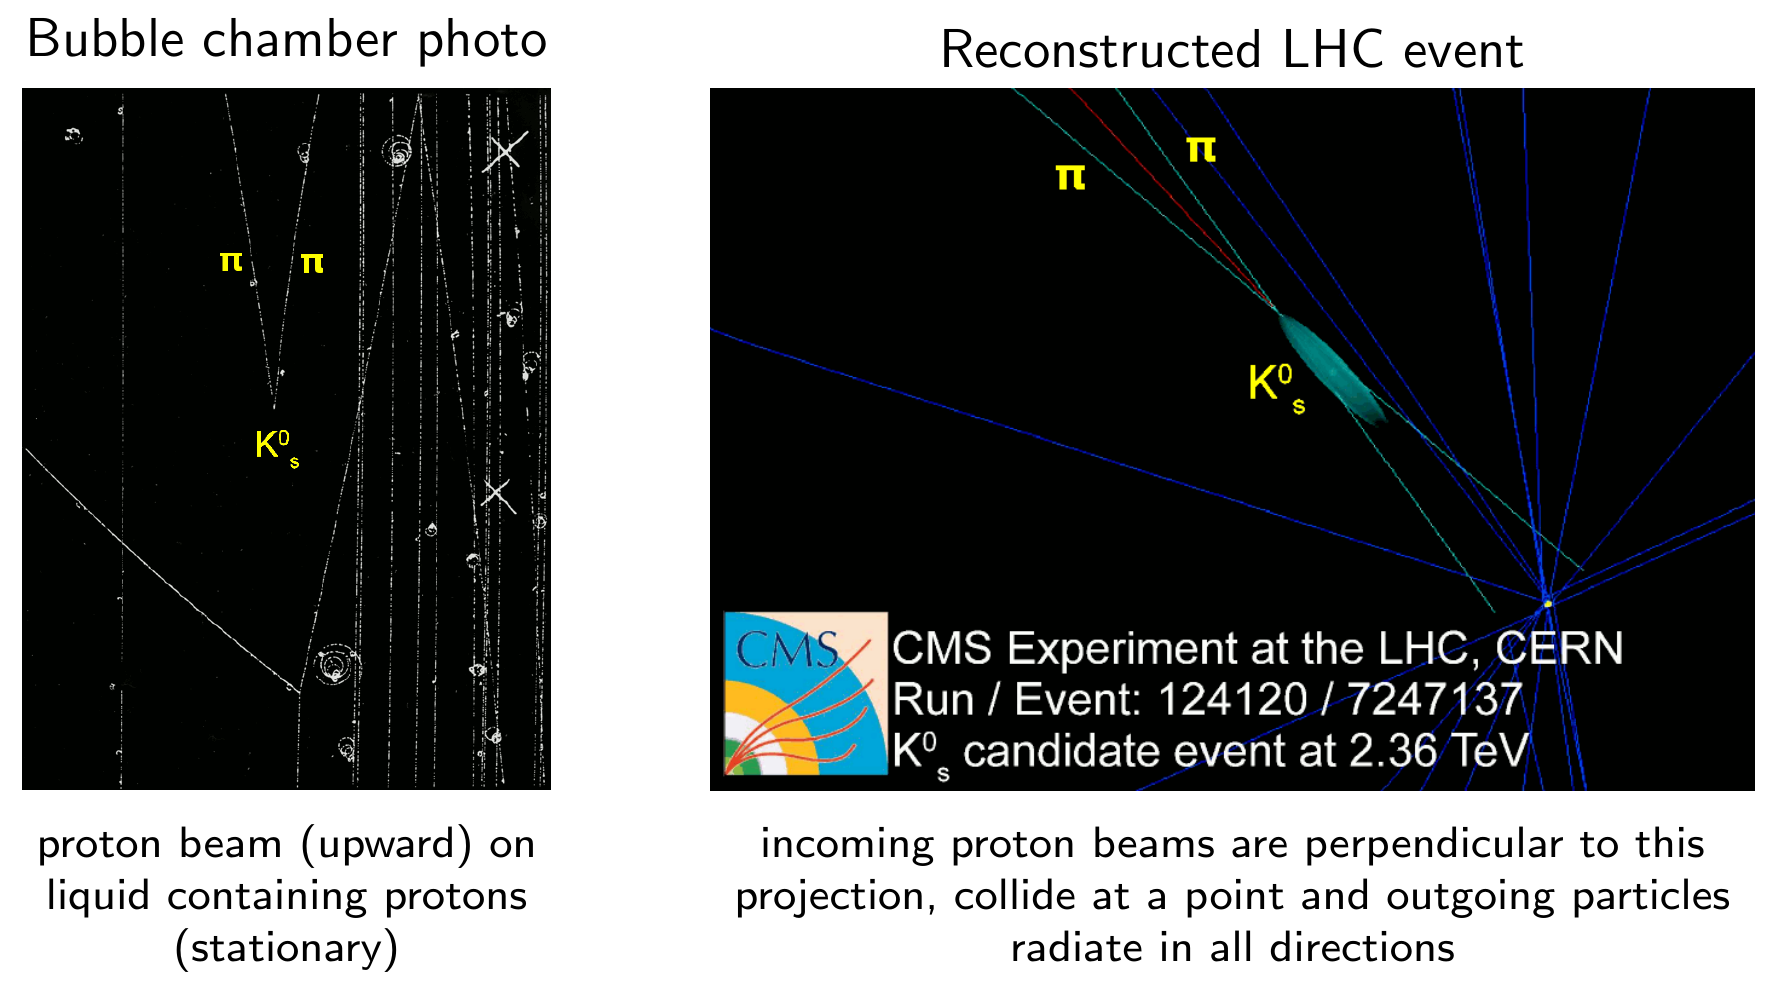
\includegraphics[width=\linewidth]{kshort.png}

%% \vspace{-7 cm}
%% \begin{uncoverenv}<2->
%% \begin{center}
%% \fcolorbox{black}{white}{\begin{minipage}{0.85\linewidth}
%% \begin{center}
%% \vspace{0.5 cm}
%% \begin{minipage}{0.85\linewidth}
%% Data are shaped like

%% \vspace{0.5 cm}
%% \only<2>{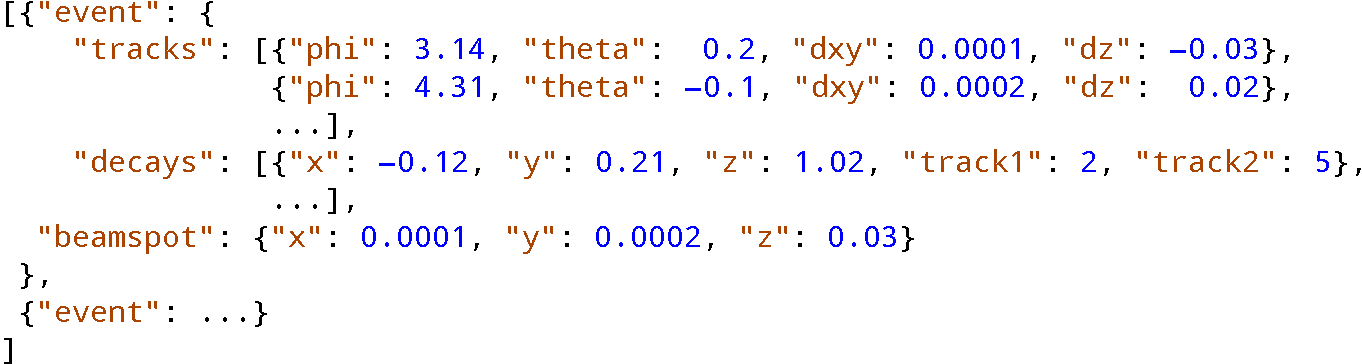
\includegraphics[width=\linewidth]{data-as-json-1.pdf}}
%% \only<3>{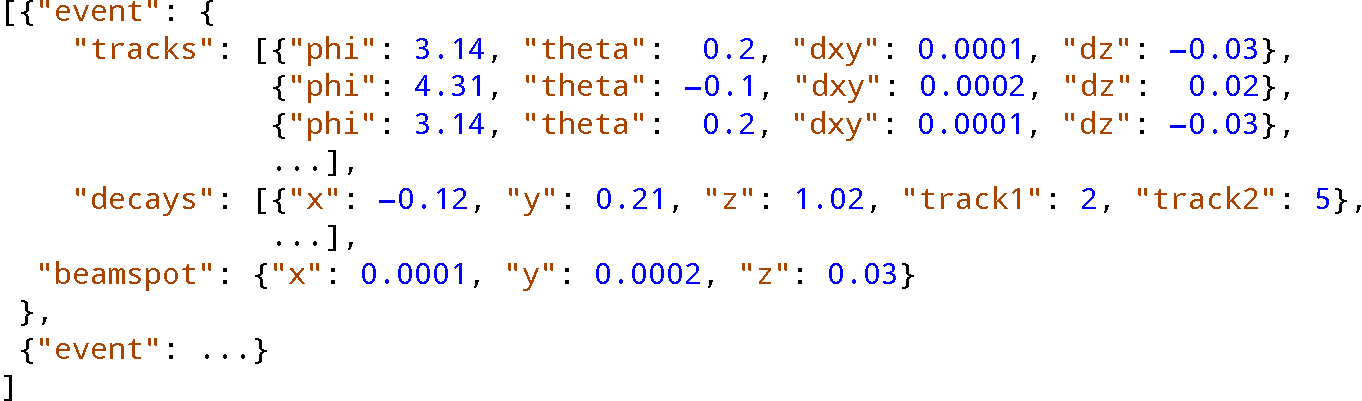
\includegraphics[width=\linewidth]{data-as-json-2.pdf}}
%% \only<4>{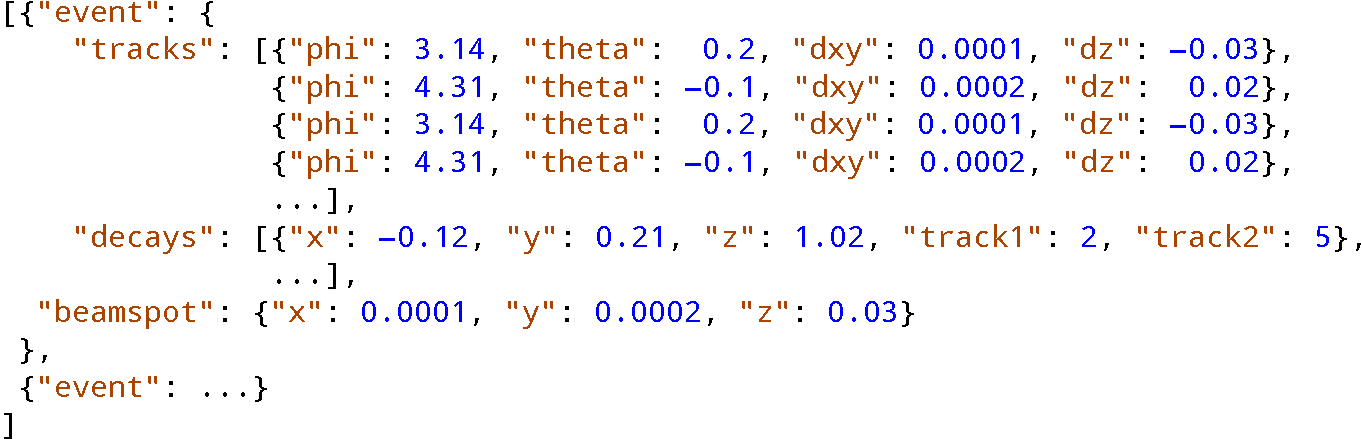
\includegraphics[width=\linewidth]{data-as-json-3.pdf}}

%% \only<3-4>{\vspace{0.5 cm}}
%% rather than a rectangular table with a fixed number of columns.
%% \end{minipage}
%% \vspace{0.5 cm}
%% \end{center}
%% \end{minipage}}
%% \end{center}
%% \end{uncoverenv}
%% \vspace{7 cm}
%% \end{frame}

%% \begin{frame}{}
%% \vspace{1.25 cm}
%% \begin{columns}[t]
%% \column{0.3\linewidth}
%% \vspace{1 cm}
%% 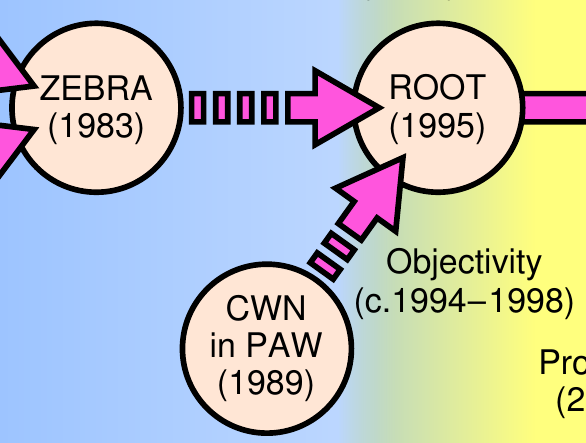
\includegraphics[width=\linewidth]{history-cropped.png}

%% \column{0.35\linewidth}
%% \underline{\large The ZEBRA heritage}

%% \vspace{0.25 cm}
%% \begin{itemize}
%% \item Arbitrary length, nested data was a requirement from the very beginning.
%% \item ZEBRA allocated these structures in FORTRAN and saved them in files.
%% \item High energy physics analyses are still batch processes on binary files.
%% \end{itemize}

%% \column{0.35\linewidth}
%% \underline{\large The CWN heritage}

%% \vspace{0.25 cm}
%% \begin{itemize}
%% \item Column-Wise Ntuples: tabular data with same-attribute values stored contiguously in memory/on disk.
%% \item {\it Much} faster to read just a few attributes, which is essential (particles have $\sim$100 attributes).
%% \end{itemize}

%% \end{columns}

%% \begin{columns}
%% \column{0.3\linewidth}

%% \column{0.75\linewidth}
%% \begin{center}
%% Though complex, it's possible to represent arbitrary length, nested data in a columnar format: ROOT (1995), Google~Dremel (2010), Apache Parquet (2013), Apache Arrow (2016).
%% \end{center}
%% \end{columns}
%% \end{frame}

%% \begin{frame}{Example of arbitrary length, nested, columnar data}
%% \vspace{0.5 cm}
%% \textcolor{darkblue}{Type/schema:} \hspace{0.28 cm}collection of\ \ {\tt\small List(List(Record(x:\ char, y:\ int)))}

%% \vspace{0.25 cm}
%% \begin{tabular}{r l}
%% \small \hspace{0.15 cm}\textcolor{darkblue}{Logical data:} & {\tt\scriptsize [\textcolor{blue}{[}\textcolor{violet}{[}(\textcolor{darkorange}{a},\textcolor{darkgreen}{1}), (\textcolor{darkorange}{b},\textcolor{darkgreen}{2}), (\textcolor{darkorange}{c},\textcolor{darkgreen}{3}), (\textcolor{darkorange}{d},\textcolor{darkgreen}{4})\textcolor{violet}{]}, \textcolor{violet}{[]}, \textcolor{violet}{[}(\textcolor{darkorange}{e},\textcolor{darkgreen}{5}), (\textcolor{darkorange}{f},\textcolor{darkgreen}{6})\textcolor{violet}{]}\textcolor{blue}{]}, \textcolor{blue}{[]}, \textcolor{blue}{[}\textcolor{violet}{[}(\textcolor{darkorange}{g},\textcolor{darkgreen}{7})\textcolor{violet}{]}\textcolor{blue}{]}]} \\
%% \small \uncover<2->{x attribute} & \uncover<2->{{\tt\scriptsize \textcolor{darkorange}{[\ \ \ a,\ \ \ \ \ b,\ \ \ \ \ c,\ \ \ \ \ d,\ \ \ \ \ \ \ \ \ \ \ e,\ \ \ \ \ f,\ \ \ \ \ \ \ \ \ \ \ \ \ g\ \ \ \ \ ]}}} \\
%% \small \uncover<2->{y attribute} & \uncover<2->{{\tt\scriptsize \textcolor{darkgreen}{[\ \ \ \ \ 1,\ \ \ \ \ 2,\ \ \ \ \ 3,\ \ \ \ \ 4,\ \ \ \ \ \ \ \ \ \ \ 5,\ \ \ \ \ 6,\ \ \ \ \ \ \ \ \ \ \ \ \ 7\ \ \ ]}}} \\
%% \small \only<3>{inner stops}\only<4->{inner offsets} & \only<3>{{\tt\scriptsize \textcolor{violet}{[\ \ \ \ \ \ \ \ \ \ \ \ \ \ \ \ \ \ \ \ \ \ \ \ \ \ \ \ 4,\ \ 4,\ \ \ \ \ \ \ \ \ \ \ \ \ \ 6,\ \ \ \ \ \ \ \ \ \ \ \ \ 7\ ]}}}\only<4->{{\tt\scriptsize \textcolor{violet}{[\ 0,\ \ \ \ \ \ \ \ \ \ \ \ \ \ \ \ \ \ \ \ \ \ \ \ \ 4,\ \ 4,\ \ \ \ \ \ \ \ \ \ \ \ \ \ 6,\ \ \ \ \ \ \ \ \ \ \ \ \ 7\ ]}}} \\
%% \small \only<3>{outer stops}\only<4->{outer offsets} & \only<3>{{\tt\scriptsize \textcolor{blue}{[\ \ \ \ \ \ \ \ \ \ \ \ \ \ \ \ \ \ \ \ \ \ \ \ \ \ \ \ \ \ \ \ \ \ \ \ \ \ \ \ \ \ \ \ \ \ \ \ \ 3,\ \ 3,\ \ \ \ \ \ \ \ \ 4]}}}\only<4->{{\tt\scriptsize \textcolor{blue}{[0,\ \ \ \ \ \ \ \ \ \ \ \ \ \ \ \ \ \ \ \ \ \ \ \ \ \ \ \ \ \ \ \ \ \ \ \ \ \ \ \ \ \ \ \ \ \ \ 3,\ \ 3,\ \ \ \ \ \ \ \ \ 4]}}} \\
%% \end{tabular}

%% \vspace{0.25 cm}
%% \begin{itemize}
%% \item<3-> Stops array is a cumulative number of items at some level of depth (see how they line up with the closing brackets?).
%% \item<4-> More convenient to have both starts and stops (``offsets'') by prepending zero.
%% \item<5-> Random access: {\tt\small data\textcolor{black}{[0]}\textcolor{blue}{[2]}\textcolor{violet}{[1]}\textcolor{darkorange}{.x}} \uncover<6->{{\tt\small = \textcolor{darkorange}{x[}\textcolor{violet}{inner[}\textcolor{blue}{outer[}0\textcolor{blue}{]} + 2\textcolor{violet}{]} + 1\textcolor{darkorange}{]} = f}.}
%% \item<7-> This is Arrow format, which is less packed than ROOT, Dremel, or Parquet.
%% \begin{itemize}
%% \item<8-> Unified disk and memory formats: ideal for memory mapping or storage-class media.
%% \item<9-> Can be extremely lightweight: when you access any memory-mapped array element, the operating system reads it and caches on demand. Faster than {\tt\small fread()}.
%% \end{itemize}
%% \end{itemize}
%% \end{frame}

%% \begin{frame}{Subject of this talk}
%% \vspace{0.5 cm}
%% We want to use zero-copy methods like memory-mapped Arrow to accelerate high-energy physics analysis--- enough to enable {\it interactive, exploratory} analysis, rather than just batch processing.

%% \vspace{0.75 cm}
%% \begin{uncoverenv}<2->
%% \textcolor{darkblue}{\it However,} the traditional method of copying serial data into runtime objects like
%% \begin{center}
%% \tt\small \textcolor{blue}{std::vector}<\textcolor{violet}{std::vector}<struct\{\textcolor{darkorange}{char x}; \textcolor{darkgreen}{int y};\}>>
%% \end{center}
%% thwarts the performance advantage of zero-copy data.
%% \end{uncoverenv}

%% \vspace{0.75 cm}
%% \begin{uncoverenv}<3->
%% \textcolor{darkblue}{\it Instead,} we are attempting to transform the user's analysis code to access the data in-place: code transformation as an alternative to deserialization.
%% \end{uncoverenv}
%% \end{frame}

%% \begin{frame}[fragile]{Example of code transformation}
%% \vspace{0.4 cm}

%% \begin{tabular}{r l}
%% \small \hspace{0.15 cm}\textcolor{darkblue}{Logical data:} & {\tt\scriptsize [\textcolor{blue}{[}\textcolor{violet}{[}(\textcolor{darkorange}{a},\textcolor{darkgreen}{1}), (\textcolor{darkorange}{b},\textcolor{darkgreen}{2}), (\textcolor{darkorange}{c},\textcolor{darkgreen}{3}), (\textcolor{darkorange}{d},\textcolor{darkgreen}{4})\textcolor{violet}{]}, \textcolor{violet}{[]}, \textcolor{violet}{[}(\textcolor{darkorange}{e},\textcolor{darkgreen}{5}), (\textcolor{darkorange}{f},\textcolor{darkgreen}{6})\textcolor{violet}{]}\textcolor{blue}{]}, \textcolor{blue}{[]}, \textcolor{blue}{[}\textcolor{violet}{[}(\textcolor{darkorange}{g},\textcolor{darkgreen}{7})\textcolor{violet}{]}\textcolor{blue}{]}]} \\
%% \small x attribute & {\tt\scriptsize \textcolor{darkorange}{[\ \ \ a,\ \ \ \ \ b,\ \ \ \ \ c,\ \ \ \ \ d,\ \ \ \ \ \ \ \ \ \ \ e,\ \ \ \ \ f,\ \ \ \ \ \ \ \ \ \ \ \ \ g\ \ \ \ \ ]}} \\
%% \small y attribute & {\tt\scriptsize \textcolor{darkgreen}{[\ \ \ \ \ 1,\ \ \ \ \ 2,\ \ \ \ \ 3,\ \ \ \ \ 4,\ \ \ \ \ \ \ \ \ \ \ 5,\ \ \ \ \ 6,\ \ \ \ \ \ \ \ \ \ \ \ \ 7\ \ \ ]}} \\
%% \small inner offsets & {\tt\scriptsize \textcolor{violet}{[\ 0,\ \ \ \ \ \ \ \ \ \ \ \ \ \ \ \ \ \ \ \ \ \ \ \ \ 4,\ \ 4,\ \ \ \ \ \ \ \ \ \ \ \ \ \ 6,\ \ \ \ \ \ \ \ \ \ \ \ \ 7\ ]}} \\
%% \small outer offsets & {\tt\scriptsize \textcolor{blue}{[0,\ \ \ \ \ \ \ \ \ \ \ \ \ \ \ \ \ \ \ \ \ \ \ \ \ \ \ \ \ \ \ \ \ \ \ \ \ \ \ \ \ \ \ \ \ \ \ 3,\ \ 3,\ \ \ \ \ \ \ \ \ 4]}} \\
%% \end{tabular}

%% \vspace{0.4 cm}
%% \begin{columns}[t]
%% \column{0.5\linewidth}
%% \underline{\large Analysis function on logical data}

%% \small
%% \begin{minted}{python}
%% for outer in data:
%%   for inner in outer:
%%     best = None  # None or rec type
%%     for rec in inner:
%%       if best is None or \
%%          rec.y > best.y:
%%         best = rec
%%     if best is not None:
%%       print(best.x)
%% \end{minted}

%% \column{0.5\linewidth}
%% \underline{\large Transformed analysis function}

%% \small
%% \begin{minted}{python}
%% for i in range(outer[-1]):
%%   best = None  # None or int type
%%   for j in range(inner[i],
%%                  inner[i + 1]):
%%     if best is None or \
%%        y[j] > y[best]:
%%       best = j
%%   if best is not None:
%%     print(x[best])
%% \end{minted}

%% \end{columns}
%% \end{frame}

%% \begin{frame}{General features of code transformation}
%% \vspace{0.5 cm}
%% \large
%% \textcolor{darkblue}{The code transformation obeys rules that can be applied recursively:}

%% \vspace{0.1 cm}
%% \begin{itemize}\setlength{\itemsep}{0.25 cm}
%% \item Objects, such as lists and records, become integer-valued indexes.
%% \item List dereferencing (e.g.\ {\tt\normalsize data[5]}) becomes offset array dereferencing.
%% \item Offset array indexes for sublists range from {\tt\normalsize outer[i]} to {\tt\normalsize outer[i~+~1]}, and list length is {\tt\normalsize (outer[i + 1] - outer[i])}.
%% \item Record dereferencing (e.g.\ {\tt\normalsize datum.x}) simply passes the index along to the nested object: {\tt\normalsize datum.x + datum.y} becomes {\tt\normalsize x[i] + y[i]}.
%% \item After transformation, there are no objects, only arrays and indexes.
%% \end{itemize}

%% \normalsize
%% \vspace{0.25 cm}
%% \uncover<2->{For our application, we have been transforming a Python abstract syntax tree (AST) and passing the result to Numba (a Python compiler for array-centric code).}

%% \vspace{0.15 cm}
%% \uncover<2->{Soon, we will attempt to encode these rules in Numba directly as a Numba extension.}
%% \end{frame}

%% \begin{frame}{Prior art}
%% \vspace{0.35 cm}
%% \begin{columns}[t]
%% \column{0.33\linewidth}
%% \mbox{ }\hfill\underline{\large Apache Drill}\hfill\mbox{ }

%% \vspace{0.25 cm}
%% \begin{itemize}
%% \item Motivating example: provides fast querying over SQL tables by transforming user queries, rather than materializing row objects.\vspace{3\baselineskip}\vspace{0.15 cm}
%% \item \textcolor{darkblue}{However,} not for arbitrary length data.
%% \end{itemize}

%% \column{0.33\linewidth}
%% \mbox{ }\hfill\underline{\large Google Flatbuffers}\hfill\mbox{ }

%% \vspace{0.25 cm}
%% \begin{itemize}
%% \item Like Google ProtoBufs, except that data are accessed in place, without deserialization.\vspace{6\baselineskip}\vspace{0.15 cm}
%% \item \textcolor{darkblue}{However,} data are not columnar.
%% \end{itemize}

%% \column{0.34\linewidth}
%% \mbox{ }\hfill\underline{\large\it Columnar Objects}\hfill\mbox{ }

%% \vspace{0.25 cm}
%% \scriptsize
%% \begin{itemize}
%% \item T.\ Mattis, J.\ Henning, P.\ Rein, R.\ Hirschfeld, M.\ Appeltauer, ``Columnar Objects: Improving the Performance of Analytical Applications,'' in {\it 2015 ACM International Symposium on New Ideas, New Paradigms, and Reflections on Programming and Software (Onward!),} 2015, pp.\ 197--210.
%% \item \normalsize Proxy objects in PyPy; similar in that PyPy is JIT-compiled.
%% \item \normalsize This is the approach we're applying to high-energy physics.
%% \end{itemize}
%% \end{columns}
%% \end{frame}

%% \begin{frame}[fragile]{Code transformation outperforms C++ with deserialization}
%% \vspace{0.25 cm}
%% \underline{Tested four realistic analysis functions on data from \only<1>{ROOT files with warmed cache}\only<2>{ROOT files or Arrow-like arrays}.}

%% \begin{columns}
%% \column{0.45\linewidth}
%% \vspace{-0.2 cm}
%% \begin{columns}
%% \column{1.1\linewidth}
%% \scriptsize
%% \begin{onlyenv}<1>
%% \begin{itemize}
%% \item \textcolor{blue}{ROOT full dataset} reconstructs objects with all attributes, including unused ones.
%% \item \textcolor{red}{ROOT selective on full} uses dummy placeholders for unused attributes.
%% \item \textcolor{darkorange}{ROOT slim dataset} uses exactly what is needed.
%% \item \textcolor{darkdarkgreen}{Code transformation on full ROOT dataset} is transformed, compiled Python code with no deserialization.
%% \end{itemize}
%% \end{onlyenv}
%% \begin{onlyenv}<2>
%% \begin{itemize}
%% \item \textcolor{darkdarkgreen}{Code transformation on full ROOT dataset} same as previous page, for scale.
%% \item \textcolor{mauve}{Same on cached arrays} releases the constraint that data originate in ROOT files, reading them from Arrow-like arrays instead.
%% \end{itemize}
%% \vspace{0.9 cm}
%% \end{onlyenv}
%% \end{columns}

%% \vspace{0.15 cm}
%% \scriptsize
%% \begin{minted}{python}
%% def mass_of_pairs(event):
%%   n = len(event.muons)
%%   for i in range(n):  # distinct pairs
%%     for j in range(i+1, n):
%%       m1 = event.muons[i]
%%       m2 = event.muons[j]
%%       mass = sqrt(
%%         2*m1.pt*m2.pt*(
%%         cosh(m1.eta - m2.eta) -
%%         cos(m1.phi - m2.phi)))
%%       fill_histogram(mass)
%% \end{minted}

%% \column{0.55\linewidth}
%% \vspace{0.1 cm}
%% \only<1>{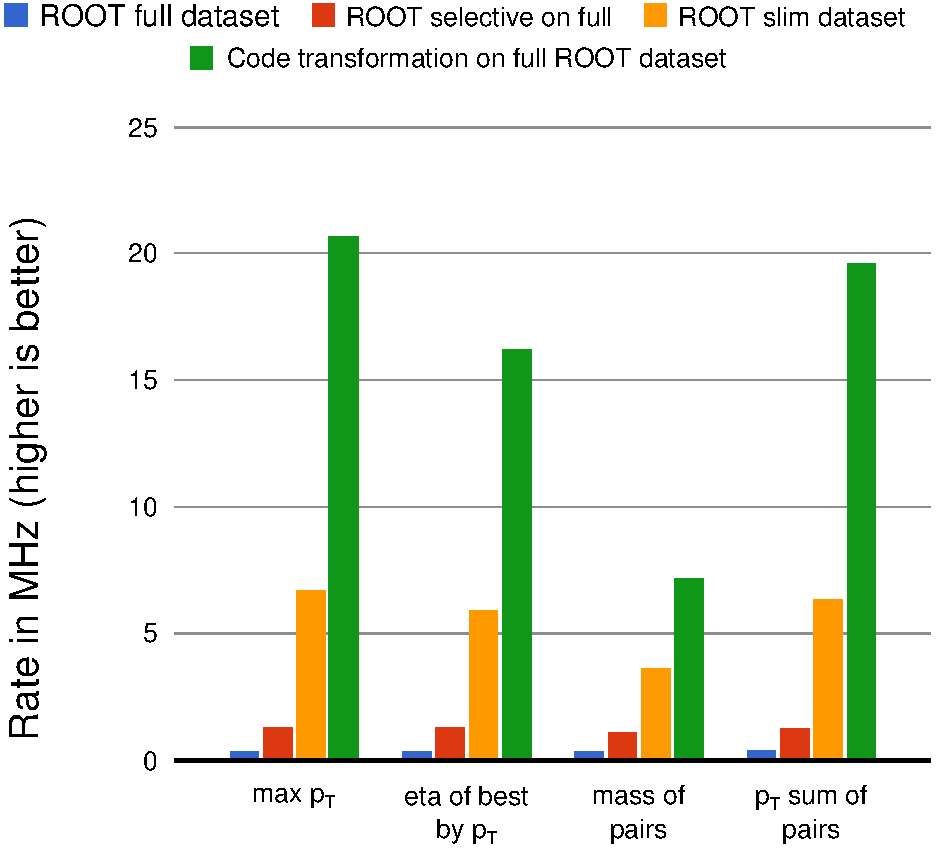
\includegraphics[width=\linewidth]{root-and-plur.pdf}}
%% \only<2>{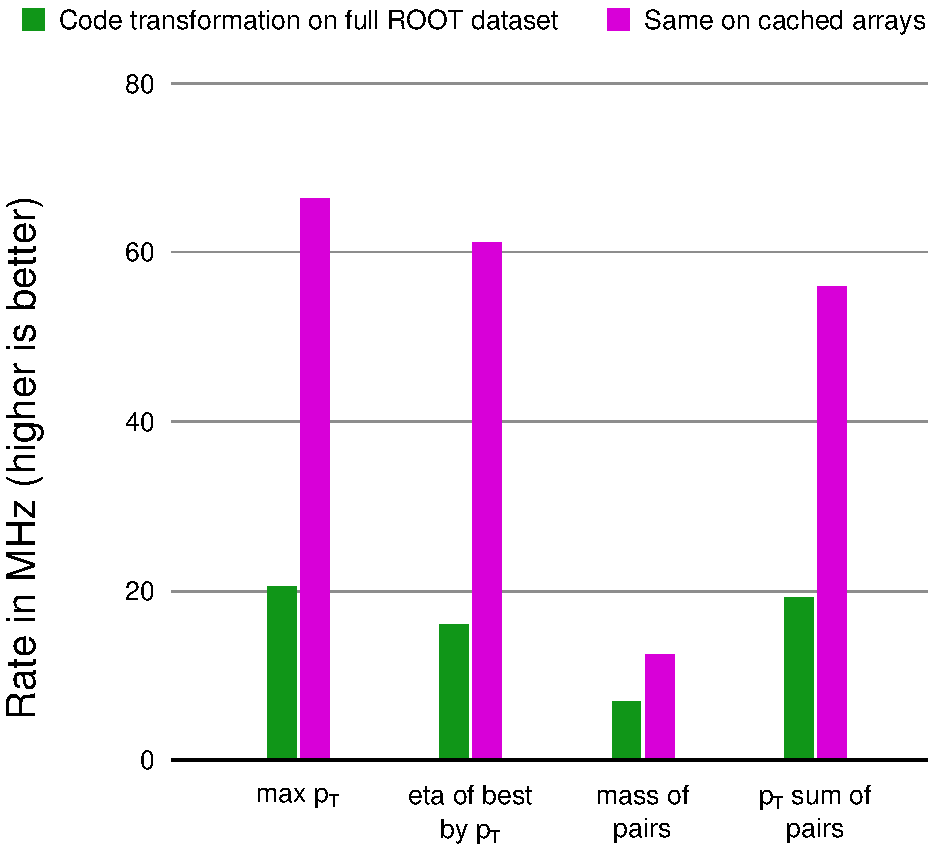
\includegraphics[width=\linewidth]{physical-media.pdf}}
%% \end{columns}
%% \end{frame}

\begin{frame}{Future work}
\vspace{0.35 cm}
\large
Although high-energy physics data are non-relational--- append-only document stores in columnar representation--- exploratory data analysis would be aided by more database-like features.

\begin{itemize}\setlength{\itemsep}{0.2 cm}
\item<2-> \textcolor{darkblue}{Resilient, distributed storage:} we're exploring the option of putting the arrays in an object store like Ceph (one array per key-value pair).
\item<3-> \textcolor{darkblue}{Distributed processing:} implementing Hadoop-style locality in the object store (hack the CRUSH algorithm?).
\item<4-> \textcolor{darkblue}{Zero-copy filtering:} expanding the data representation (next page) would allow subsets to be expressed without copying list contents, like a database stencil.
\item<5-> \textcolor{darkblue}{Database-style indexing:} same extension would allow us to sort substructures by a primary key without altering logical order.
\end{itemize}
\end{frame}


\end{document}
